\section{Scalability Testing}

\subsection{Definition of Scalability}
In a large scale environment, a choreography must be able to attend different scenario sizes. Web Services Choreographies will probably have some periods that will require more resources that it is usual to maintain its performance.  Suppose that a specific choreography, for example, receives usually N requests per second but, in some specific times, receives 10N requests. It must have tolerance to this increase of access quickly.

To support this issue, we may increase its system capability between this period of high demand. We want to have the same performance that we had previously. Therefore, we must know how much of resources we should increase to achieve this goal.  Each choreography will have its particular solution. This will depends on how the choreography is implemented. Bad choreographies architectures will need to increase a lot to achieve that, someones won't even achieve that.

For instance, in the example above, we could increase the resources in the same scale that the number of access increased to gain the same performance. However, only that will not assure we will perform that, i.e.  the choreography may have a bottleneck that will not disappear if we add more resources. Thus, we also must pay attention with the implementation of the choreography. We gain scalability with the collaboration of the hardware and the software. 

Architectures that achieved the same performance by increasing the architecture capability with the same proportion as the increase of the problem size are scalable [\citet{QUINN}]. For \citet{LAW}, a simulation is scalable if the improvements in simulation capability express in direct proportion improvements in architectural capability. However, these definitions just say if an application is scalable or not. Consequently, we can not compare the scalability of two applications by saying that one is more scalable than the other. To conclude how scalable an application is, we need to quantify it. Law quantify simulation scalability in a mathematical model, based on two capabilities, simulation and architectural. 

\subsection{Quantifying Scalability}

A simulation is built on a set of values that describe its state, this is called measures of interest. We also know it must meet a set of performance requirements. A simulation attain acceptable performance if it execute with correctness and satisfy the performance requirement. For instance, in a web service stress simulation, the number of requests per second is a measure of interest, and a performance requirement is the average response time. If the simulation do not have a minimum satisfactory response time average with correct responses, it did not achieve acceptable performance. 

Based on the measures of interested and the performance requirements, we can tell the complexity of the problem. The author define the complexity size with the function $S(n_{1}..n_{s})$, where $n_{1}$ to $n_{s}$ is a set of $s$ variables. This variables are measures of interested and performance requirements inputs. Its assumed that if one of this variables increase, the simulation size function will increase or at least stay the same, but never decrease. There are different ways to define the complexity of a problem. It depends on the characteristics we want to analyze.

We've seen performance as a requirement, however we may also be interested in its precise values. For example, the memory usage may be a metric that we want to minimize even if we have not defined what is the maximum value that it can achieve. Thus, Law defines a function that characterize the performance metrics, $M(m_{1}..m_{q})$, where $m_{1}$ to $m_{q}$ is a set of $q$ performance metrics. If a performance metric increase, its assumed that the performance improves. We can reverse the metrics that do not behave this way. If $Y$ is the memory usage metric, we can pass $\frac{1}{Y}$ as input. With these definition we conclude that a simulation capability is the relation of the functions $S$ and $M$, defined as $C(S,M) = SM$.

As said previously, to measure scalability we need also to quantify the architectural capability. The inputs that we need to achieve this are the architecture characteristics, such as the CPU clock speed. The function $P(h_{1}..h_{p})$ describes it, where $h_{1}$ to $h_{p}$ are the variables that represent the measures of the architecture.

With the definition of these two functions, we choose a architecture with capability $P_{1}$. $C_{1}(S,M)$ will be choose as the largest value that the architecture of capability $P_{1}$ can compute the problem with correctness and meet all the performance requirements for every element of the simulation capability domain. Therefore, $k = \frac{C_{1}(S,M)}{P_{1}}$, is the best ratio between simulation capability and architectural capability that is achievable with the chosen system architecture.

Let $C_{i}$ and $P_{i}$ be capabilities $i$ times greater than $C_{1}$ and $P_{1}$, respectively. Therefore, the author defines scalability as the largest real-value $j$ such as $\frac{C_{i}(S,M)}{P_{i}} \geq k$ for every $i$ in the real-value interval $[1,j]$ and $P_{i}$ can compute the problem of complexity size $C_{i}(S,M)$ with correctness and meet all the performance requirements. With these definition we can are verify the interval where the ratio between the simulation capability and the architectural capability stays at least equal as it was initially. If $j = \infty$, we say that the system is fully scalable.

This definition, however, has some limitations as pointed out by Law. One of them is  difficulty to define a architectural capability function that express the exact importance between each hardware characteristic. For example, a system with 512MB of RAM and 100GHz of CPU may have the same capability than one with 256MB and 200GHz of CPU. Another one is about the highly dependency on the definition of the architectural and simulation capabilities in the scalability function. This means that, the same system can have different ranges of scalability depending on how we define these functions. The point here is that is very difficult to quantify the variables P and C. Therefore, If we can not quantify properly them, we won't be able to quantify the scalability of a system. 

These restrictions show us that scalability is something relative, a system may have different ranges of scalability depending on the importance that we gave to its elements. However, despite this limitations, we can adapt it to something more usable. We can use the scalability function to compare two systems with the same architectural and simulation capabilities. We, also, limit the number of the capability functions input to one. Let $c$ be the input for the simulation capability function $C_{i}$ and $h$ for the architectural capability function. Thus, we can conclude if a system is more scalable then another based on these two variables. Law, presents the final definition of scalability as the largest real-value $j$ such that $\frac{C_{i}(c)}{P_{i}(h)} \geq k$ for every i in the real-value interval $[1.0, j]$ and $P_{i}(h)$ can compute the problem of complexity size $C_{i}(c)$ with correctness and meet all the performance requirements.

With these description, the author narrow the scalability comparison of two system relative to a specific aspect of the simulation and architectural. For example, we choose $c$ as the size of data send per request to a web service, and h as the RAM of the web service hardware. Then we can compare if one system has more scalability than the other in terms of space usage. 

\subsection{Types of Scalability}
With the definition presented in the subsection above, we conclude that are different ways to examine the scalability of a system. \cite{BONDI} presents four types of scalability that we can observe:

\begin{description}
\item[Load scalability] A system has more load scalability if it behaves properly with light, moderate or heavy loads. In this case, the word \emph{properly} is related to functional and non-functional aspects, such as resource contention, excessive of delay, and ineffective memory consumption. Thus, to measure the load scalability of a system using the scalability function, we would use, for instance,  number of request per second as the input for the simulation capability function, the number o processor as the input for the architectural capability, and fixing the response time average as a performance metric.
\item[Space scalability]  A system has more space scalability if its memory requirements grows largely when the number of supported items increase. For example, measuring the scalability based on the data size sent per request as an input for the simulation capability function, the RAM of the system hardware, and fixing the percentage of RAM used as a performance metric.
\item[Space-time scalability] A system has more space-time scalability if it function properly, i.e., without much delays, when the number of its objects increase. If a search system takes more time to find an information because of the increasing of data storage, even if its hardware resources has grown too, we conclude that it does not have space-time scalability.
\item[Structural scalability] A system is structural scalable if it does not prevents the increasing of objects that it encompasses. For example, if a peer-to-peer system has a maximum number of nodes that it support and another has not, then the latter is more structural scalable than the former.
\end{description}

These types of scalability gives us a direction of what we need to observe when comparing the scalability of the systems. Its important to note that they are, sometimes, dependent from each other. A system that needs space-time scalability may also needs space scalability because the huge grown of memory might cause a delay to find information.

\subsection{Related Works}

\cite{STAS} present the Scalability Testing and Analysis System (STAS), which is a tool that support users for running scalability analysis of algorithms and system. STAS analysis scalability using the metric \emph{isospeed-efficiency scalability}, also known as \emph{isospeed-e}. 

The architecture capability used in this metric is the sum of the supported speeds of all system nodes. Let $h_{i}$ be the supported speed of a specific node $i$, then the architecture capability of the system is $P(n) = \sum_{i=1}^{n} h_i$ , where $n$ is the number of nodes. 

A function that characterize the complexity of the problem, defined by the user, combined with the execution time, which is the performance metric, results the simulation capability function $C = \frac{S}{T}$, where $S$ is the value that represents the complexity of the problem and $T$ is the execution time metric. Therefore the scalability function is defined as $\frac{C}{P}$.

STAS is composed by four components as shown in Figure \ref{stasarchitecture}: system characterization component, algorithm pre-analysis component, scalability tester component, and scalability analyzer component.

\begin{figure}[htbp]
\begin{center}
	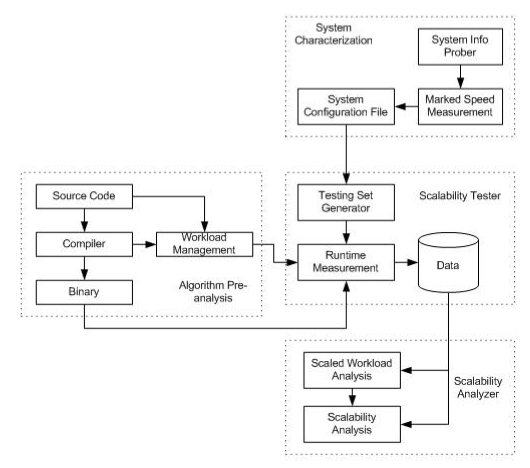
\includegraphics[scale=0.6]{images/stasarchitecture}
\caption{STAS Architecture [\cite{STAS}]}
\label{stasarchitecture}
\end{center}
\end{figure}

The system characterization component is responsible for calculating the supported speed of each node available by measuring their FLOPS. The algorithm pre-analysis component is responsible for calculating the problem complexity defined by the user. 

The scalability tester component executes the application and measure the time of the execution.  It calculates $C_1$ by applying the function described above with the values obtained. After that, it execute the application after doubling the number of nodes and the parameter of the complexity problem function. $C_2$ is obtained with the execution information. This process is done until it reaches the maximum number of nodes available. The results are compared by the scalability analyzer component that concludes how scalable the application is.










